\documentclass{standalone}
\usepackage{pgfplots}
\pgfplotsset{compat=1.13}
\usepackage{amsmath}
\colorlet{paleBlue}{blue!10!white}

\begin{document}

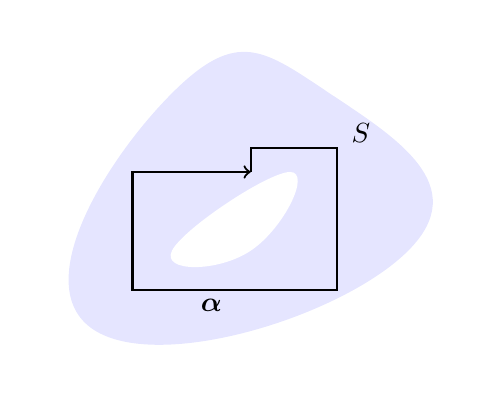
\begin{tikzpicture}
    \fill[paleBlue] plot [smooth cycle, tension=1] coordinates {(0,0) (1,3) (3,3) (4,1)};
    \fill[white] plot [smooth cycle, tension=1] coordinates {(1,1) (2,1) (2.5,2)};
    % \fill[paleBlue] plot [smooth cycle, tension=1] coordinates {(0,0) (1,3)  (3,3) (4,1)};
    \draw[->,thick] (2,2) -- (2,2.3) -- (3.1,2.3) -- (3.1,.5) -- (.5,.5) -- (.5,2) -- (2,2);
    \node at (3.4,2.5){\(S\)};
    \node at (1.5,0.3){\(\boldsymbol\alpha\)};
\end{tikzpicture}

\end{document}